\documentclass[main.tex]{subfiles}
\begin{document}
\chapter{Introduction}
\label{chapter:intro}
The standard model of particle physics (SM) is our current best working
theory that describes the phenomenon we observe, for  example,
 at collider experiments.
The large hadron collider (LHC) is a high energy proton-proton
collider experiment that allows us to study the fundamental particles
laid out in the standard model.

The interaction of these fundamental particles are described
by scattering amplitudes. The standard model allows us to
calculate these amplitudes, or matrix elements, from first
principles. A key challenge in the past few decades has been
to compute these matrix elements for increasing number of
final state particles and for higher orders in perturbative
expansions in fixed order calculations. Although there
has been tremendous progress in this sector a complication
that naturally arises is that the evaluation of these matrix
elements becomes increasingly time-consuming due to their
algebraic complexity.

The topic of this thesis is to apply modern machine learning
techniques to reduce the time spent evaluating these
complex matrix elements. Considering the physical properties
of these matrix elements allows us to implement physics
knowledge into these machine learning algorithms giving
us higher levels of performance than would otherwise be
achievable.

The structure of this thesis is as follows: in Chapter~\ref{chapter:intro}
I will recap the necessary concepts from the standard
model, in particular, on quantum chromodynamics (QCD), the sector
which governs the behaviour of quarks and gluons. Furthermore,
the relationship between theory and experiment will be elaborated on.

In Chapter~\ref{chapter:qcd} I will discuss the challenges that arise
in fixed order perturbative calculations and the current methods
that have been adopted in the community to deal with them. These
methods also form the basis of our physics knowledge which we
embed into the machine learning algorithm. This procedure is 
described in detail in Chapter~\ref{chapter:fame1} for electron-positron
annihilation for tree-level matrix element emulation.
A similar philosophy is applied in Chapter~\ref{chapter:fame2}
where next-to-leading order QCD k-factors are emulated.
These two chapters discuss in detail the procedure for
electron-positron annihilation, however, the most relevant
experiment currently is the LHC which is colliding protons.
The extension to hadron-hadron colliders is detailed in
Chapter~\ref{chapter:fame3} where we explore using the
emulator in a novel implementation to replace traditional
matrix element providers in the event generator SHERPA.

Finally, I will conclude the thesis in Chapter~\ref{chapter:conclusion}.

\section{The Standard Model of particle physics}
    The Standard Model of particle physics (SM) is our current
    best working theory to describe all known elementary particles
    as well as three of the four fundamental forces. Developed
    predominantly in the latter half of the 20th century, it is
    one of the most well tested theories we have in science today.
    Some highlights include the highly precise predictions of the
    anomalous magnetic moment of the electron, agreeing with experimental
    measurements to more than 10 significant figures \cite{Aoyama:2017uqe}.
    and the discovery of the Higgs boson in 2012 by the ATLAS \cite{ATLAS:2012yve}
    and CMS experiments \cite{CMS:2012qbp} at the Large Hadron Collider
    (LHC) which was theorised decades prior.

    The SM is a gauge quantum field theory (QFT) where particles
    are described as excitations in quantum fields. It can be specified
    by the gauge group
    \begin{equation}\label{eqn:SM_gauge}
        \mathrm{SU}(3)_{C} \times \mathrm{SU}(2)_{L} \times \mathrm{U}(1)_{Y}\, ,
    \end{equation}
    where subscripts denote the charges of the gauge groups. The first gauge
    group with colour charge $C$ describes the interactions of the
    strong force within the theory of quantum chronodynamics (QCD), which we
    will elaborate more on in the next section. The second
    and third gauge groups represent the electroweak sector of the SM with
    charges $L$ for left and $Y$ for hypercharge. Under electroweak
    spontaneous symmetry breaking (EWSB), this product becomes
    \begin{equation}\label{eqn:SM_SSB}
        \mathrm{SU}(2)_{L} \times \mathrm{U}(1)_{Y} \xrightarrow{\mathrm{EWSB}} \mathrm{U}(1)_{\mathrm{EM}} \, ,
    \end{equation}
    giving rise to the electromagnetic and weak forces we observe.
    The effect of gravity is considered to be negligible on the scales
    considered in the SM and so it is not described.
    Each of the three fundamental forces described by the SM is mediated
    by the exchange of a gauge boson. The gauge bosons mediating the strong
    and EM force are the massless gluon $g$ and massless photon $\gamma$,
    respectively. For the weak force the gauge bosons are the $W^{\pm}$
    and $Z^{0}$ bosons which attain a mass through the Higgs mechanism \cite{Englert:1964et,Higgs:1964pj,Guralnik:1964eu}
    during EWSB, which elucidates the Higgs boson $H$.

    The matter content of the SM consists of fermions which can be split
    into quarks and leptons. Quarks are massive and experience the strong,
    weak, and EM force. Leptons are defined by their lack of colour charge,
    meaning they do not experience the strong force. Leptons can be separated
    into charged leptons (electron $e$, muon $\mu$, tau $\tau$
    and their antiparticles) which experience the weak and EM force, and 
    neutrinos (electron neutrino $\nu_{e}$, muon neutrino $\nu_{\mu}$, tau
    neutrino $\nu_{\tau}$ and their antiparticles) which only experience the
    weak force. Neutrinos are massless in the SM but this is not a requirement
    of the model. In fact they have been observed to have mass (cittation here).

    The particle content of the SM is summarised in Figure \ref{fig:SM_particles}
    showing the quarks, leptons and bosons along with their masses, charges
    and spin.
    \begin{figure}
        % 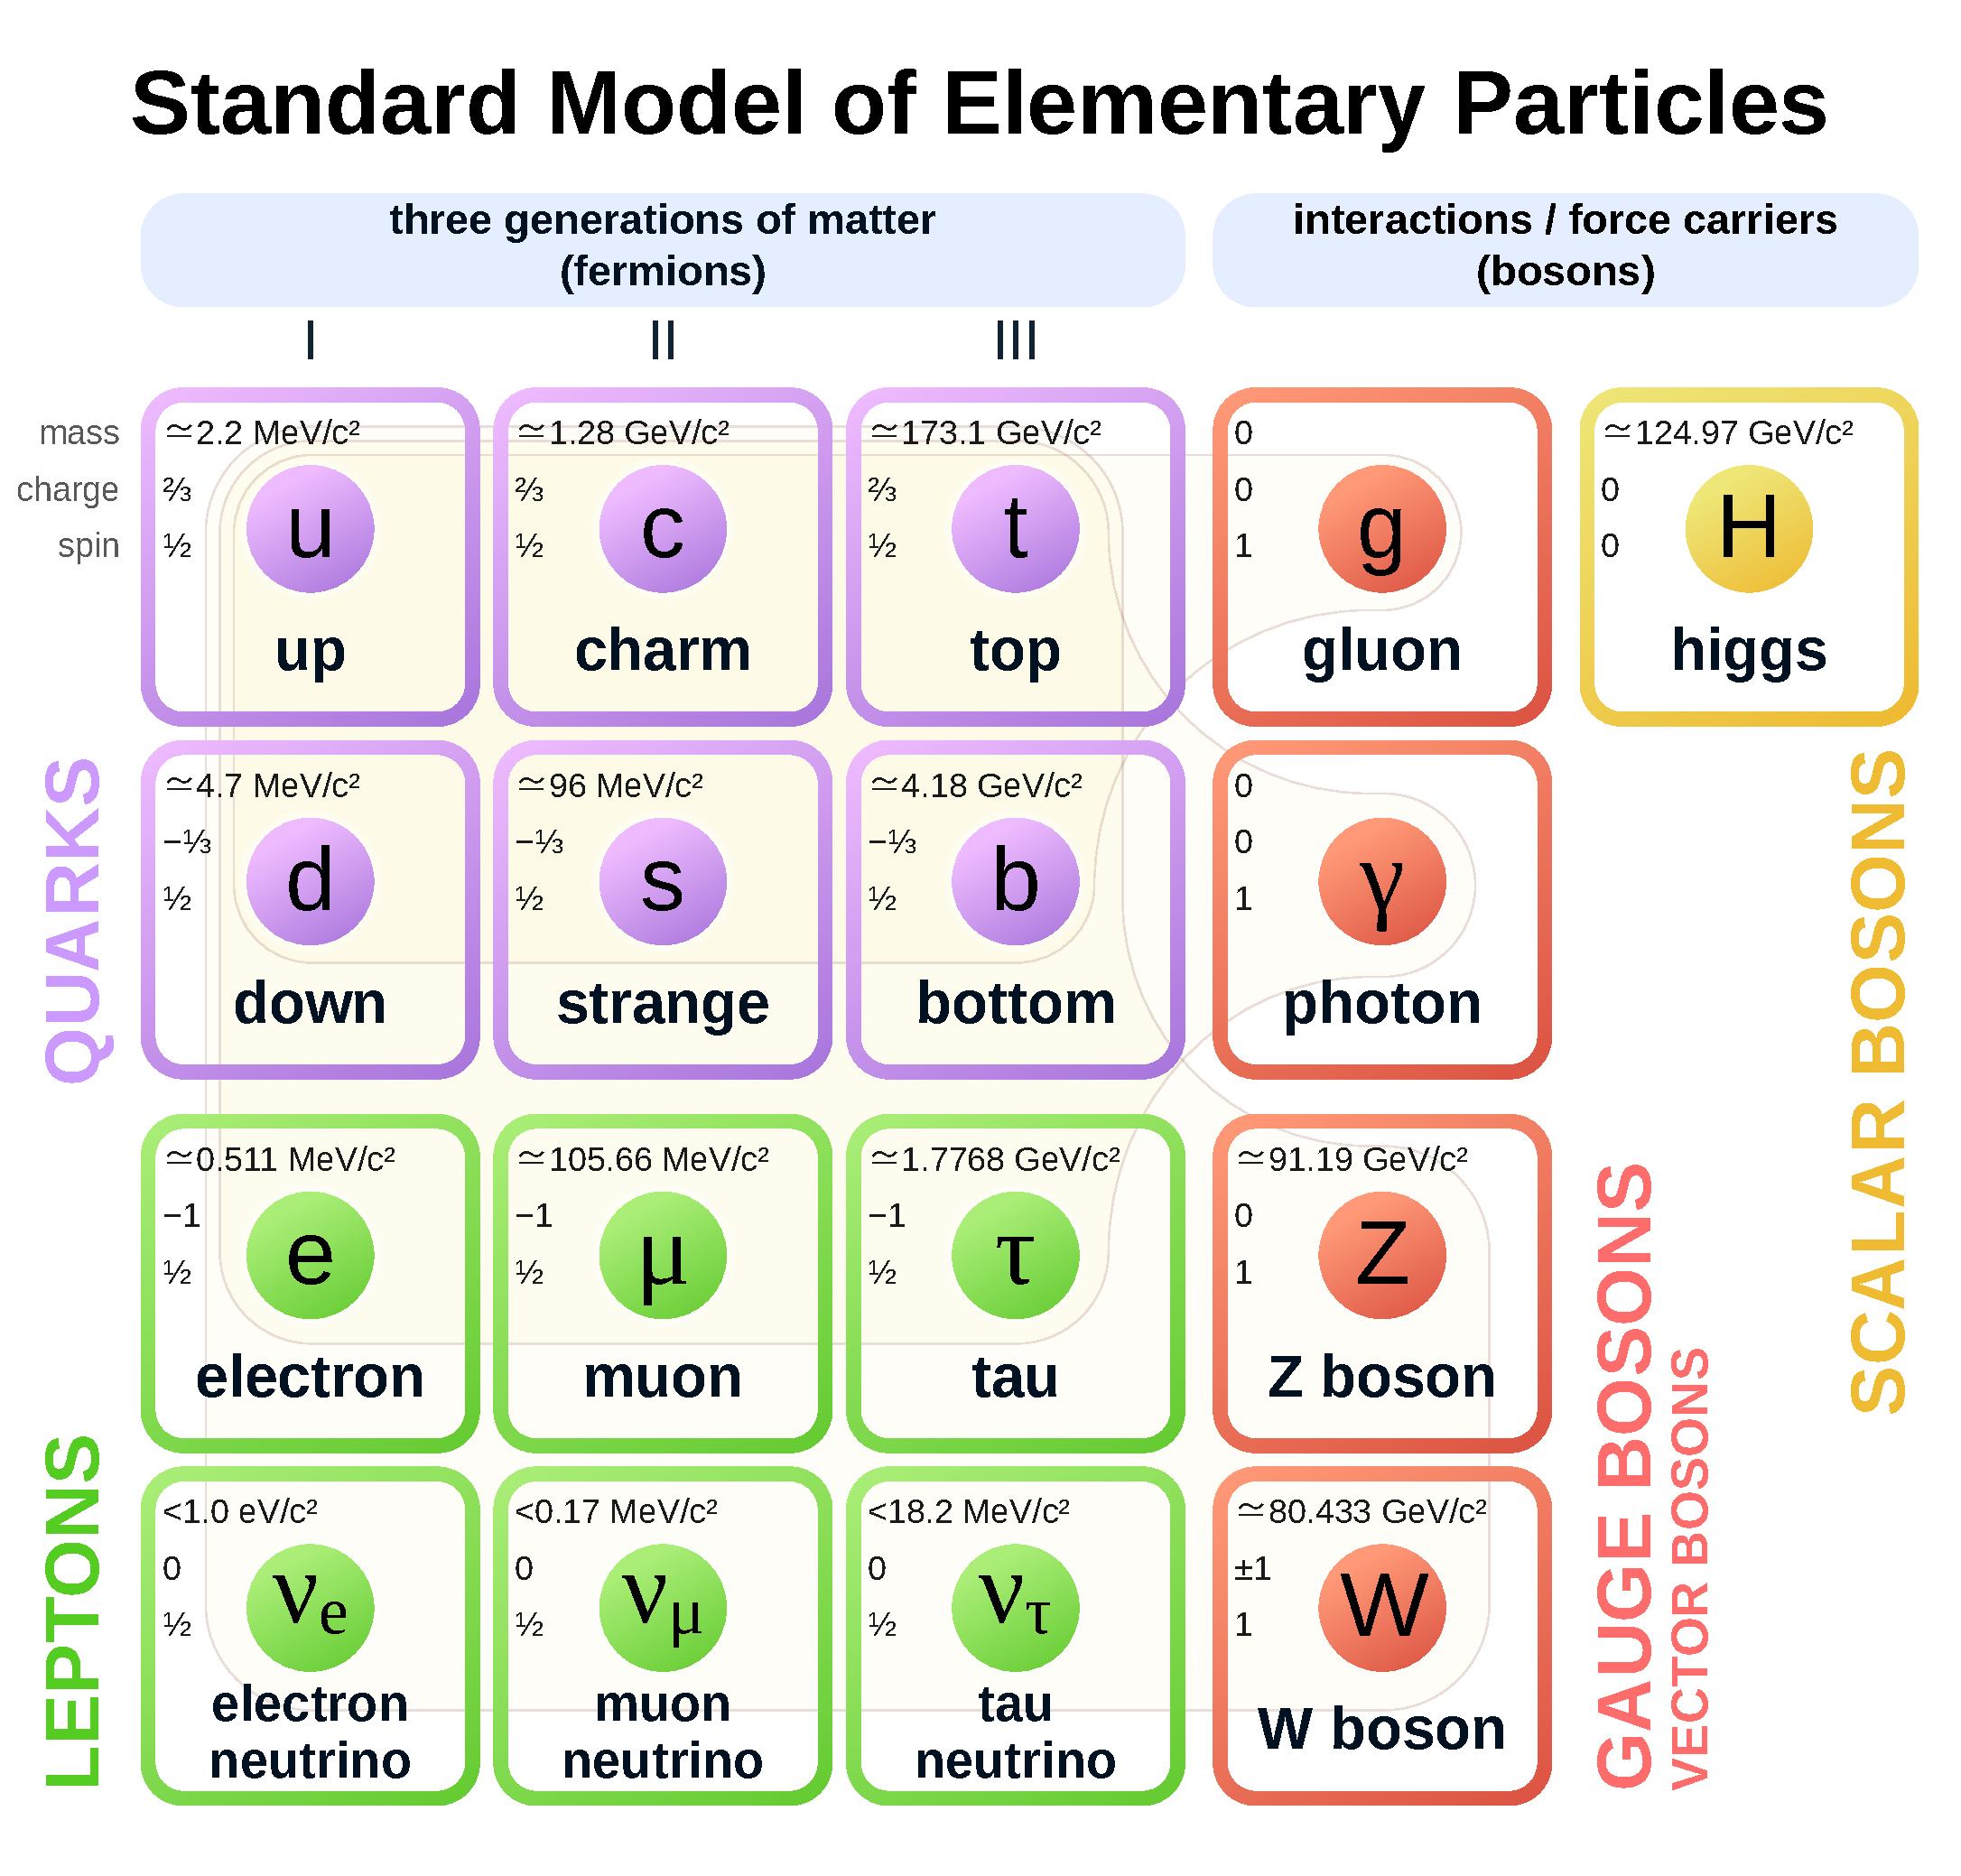
\includegraphics[width=\linewidth]{introduction/sm_particles.pdf}
        \caption{Particle content of the SM split into quarks, leptons,
        gauge bosons and scalar bosons. The columns for the fermions depict
        the three different generations. Masses, electric charge, and spin
        are given for each particle. The yellow contours indicate the coupling
        of bosons to fermions, illustrating the forces experienced by the
        fermions inside the contour. Figure reference \cite{SM_figure}.}
        \label{fig:SM_particles}
    \end{figure}
    The interactions of these fields are governed by the SM Lagrangian
    \footnote{technically Lagrangian density but we use the terms
    Lagrangian and Lagrangian density interchangeably}
    which can be written as
    \begin{equation}\label{eqn:L_SM}
        \mathcal{L}_{\mathrm{SM}} = \mathcal{L}_{\mathrm{gauge}} + \mathcal{L}_{\mathrm{fermion}} + \mathcal{L}_{\mathrm{Higgs}} + \mathcal{L}_{\mathrm{Yukawa}} + \mathcal{L}_{\mathrm{GF}} + \mathcal{L}_{\mathrm{ghost}} \, ,
    \end{equation}
    where $\mathcal{L}_{\mathrm{gauge}}$ describes the gauge fields,
    $\mathcal{L}_{\mathrm{fermion}}$ describes how fermions interact with
    gauge fields as well as their kinetic terms,
    $\mathcal{L}_{\mathrm{Higgs}}$ describes the Higgs field,
    $\mathcal{L}_{\mathrm{Yukawa}}$ describes the interaction between the Higgs
    field and fermions,
    $\mathcal{L}_{\mathrm{GF}}$ is a gauge fixing term,
    and $\mathcal{L}_{\mathrm{ghost}}$ is a ghost term.
    The last two terms are required to remove unphysical degrees of freedom
    when gauge fixing the theory.
    All terms in the SM Lagrangian are invariant under local transformations
    of the gauge group (\ref{eqn:SM_gauge}).

    In the following section we will focus on the gauge, fermion, gauge-fixing
    and ghost Lagrangian terms in the framework of QCD as that will be the
    most relevant sector for this thesis. The remaining terms are discussed at
    length in standard reference texts \cite{Peskin:1995ev,Schwartz:2014sze,Romao:2012pq}.


\section{Introduction to quantum chromodynamics}
    Quantum chronodynamics (QCD) is the sector of the SM that
    describes the strong interaction. 
    QCD is a non-Abelian gauge theory with gauge group
    $\mathrm{SU}(3)_{C}$ where the charge is named colour.
    The gauge and fermion part of the QCD Lagrangian is
    \begin{equation}\label{eqn:L_QCD}
        \mathcal{L}_{\mathrm{QCD}} = -\dfrac{1}{4}F^{a}_{\mu\nu}F^{a, \, \mu\nu}
        + \sum_{f} \bar{\psi}_{i}^{f}(\mathrm{i}\slashed{D}_{ij} - \delta_{ij}m_{f})\psi_{j}^{f} \, ,
    \end{equation}
    where twice repeated indices are summed over.
    The fields $\psi_{i}^{f}$ ($\bar{\psi}_{i}^{f}$) are the fermions (antifermions),
    representing quarks (antiquarks) with flavours $f$: 
    up $u$, down $d$, strange $s$, charm $c$, top $t$, and bottom $b$,
    with masses $m_{f}$. They transform under the fundamental
    representation with indices $i, j \in \{1, 2, 3\}$, named colour indices.
    The gauge fields $A^{a}_{\mu}$, corresponding to gluons, 
    appear in the quark covariant derivative
    \begin{equation}\label{eqn:covariant_deriv}
        (D_{\mu})_{ij} = \delta_{ij}\partial_{\mu} - ig_{\mathrm{s}}T^{a}_{ij}A^{a}_{\mu} \, ,
    \end{equation}
    and the gauge field strength tensor
    \begin{equation}\label{eqn:F_munu}
        F^{a}_{\mu\nu} = \partial_{\mu}A^{a}_{\nu} - \partial_{\nu}A^{a}_{\mu} + g_{\mathrm{s}} f^{abc}A^{b}_{\mu}A^{c}_{\nu} \, .
    \end{equation}
    Gauge fields transform under the adjoint representation, meaning
    the adjoint indices $a,b,c \in \{1,...,8\}$. $T^{a}_{ij}$ are the
    group generators in a fundamental representation. In SU(3) it is
    common to write the group generators as
    \begin{equation}\label{eqn:group_generators}
        T^{a}_{ij} = \dfrac{1}{2}\lambda^{a}_{ij}
    \end{equation}
    where $\lambda^{a}_{ij}$ are the Gell-Mann matrices \cite{Gell-Mann:1962yej}.
    The generators of the group have to obey the Lie algebra
    \begin{equation}\label{eqn:lie_algebra}
        [T^{a}, T^{b}] = \mathrm{i}f^{abc}T^{c} \, ,
    \end{equation}
    where $f^{abc}$ are the structure constants of SU(3).
    The gauge coupling of the group $g_{\mathrm{s}}$
    is a dimensionless free parameter of the theory.
    It is common to use the strong coupling constant
    instead, 
    \begin{equation}\label{eqn:alpha_s}
        \alpha_{\mathrm{s}} = \dfrac{g_{\mathrm{s}}^{2}}{4\pi} \, .
    \end{equation}
    The strong coupling constant, is not constant, but
    is dependent on the energy scale of the process, $\mu$.
    The behaviour of $\alpha_{\mathrm{s}}$
    is governed by the Callan-Symanzik \cite{Callan:1970yg,Symanzik:1970rt}
    $\beta$-function
    \begin{equation}\label{eqn:beta_fn}
        \mu^{2} \dfrac{\partial \alpha_{\mathrm{s}}(\mu^{2})}{\partial \mu^{2}} = \beta(\alpha_{\mathrm{s}}) \, ,
    \end{equation}
    where the $\beta$-function can be written as a perturbative
    expansion in $\alpha_{\mathrm{s}}$
    \begin{equation}\label{eqn:beta_series}
        -\beta(\alpha_{\mathrm{s}}) = \sum_{n=0}^{\infty}\dfrac{\alpha_{\mathrm{s}}^{n+2}}{(4\pi)^{n+1}} \beta_{n}\, .
    \end{equation}
    where the coefficients $\beta_{n}$ have been computed
    up to fifth order \cite{Baikov:2016tgj,Luthe:2017ttg}.
    The coefficients computed up to this point have been
    strictly positive, meaning that $\alpha_{\mathrm{s}}$
    decreases with increasing energy due to the minus sign
    in (\ref{eqn:beta_series}), a property known as
    asymptotic freedom \cite{Gross:1973id,Politzer:1973fx}.
    The solution to (\ref{eqn:beta_fn}) to first order
    is
    \begin{equation}\label{eqn:1l_alpha}
        \alpha_{\mathrm{s}}(\mu^{2}) = \dfrac{1}{\frac{\beta_{0}}{4\pi}\log(\frac{\mu^{2}}{\Lambda_{\mathrm{QCD}}^{2}})} \, ,
    \end{equation}
    where $\Lambda_{\mathrm{QCD}}$ is the QCD scale,
    the scale at which $\alpha_{\mathrm{s}}$ becomes
    large enough that perturbation theory breaks down.
    The running of the coupling constant has been
    observed experimentally as can be seen in Figure~\ref{fig:alpha_s_running}.
    \begin{figure}
        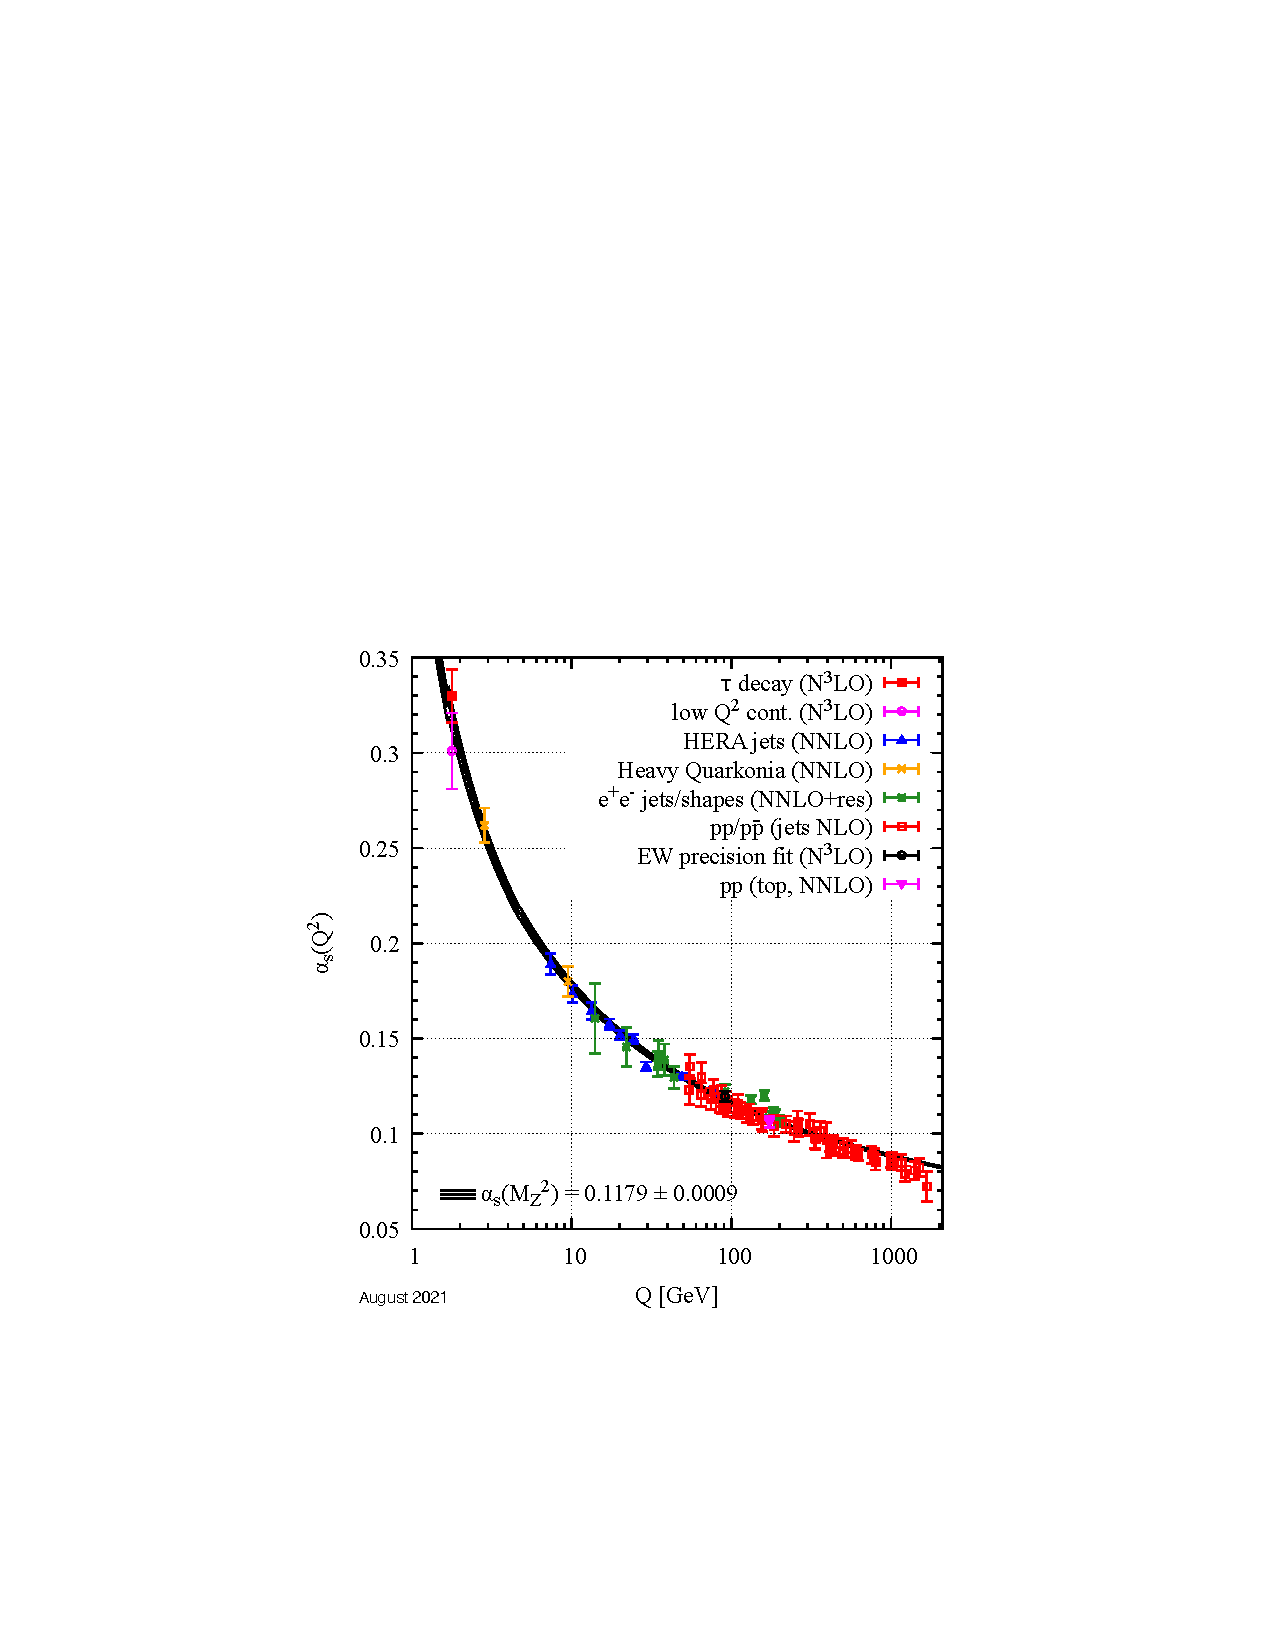
\includegraphics{alpha_s_running.pdf}
        \caption{The running of the strong coupling constant $\alpha_{\mathrm{s}}$,
        as determined by experiments, with QCD theory prediction in black.
        Figure reference \cite{Workman:2022ynf}.}
        \label{fig:alpha_s_running}
    \end{figure}
    Another consequence of the running coupling
    is colour confinement, in which quarks and
    gluons cannot exist as free particles. Due
    to the increasing strength of coupling at low
    energies, quarks and gluons are forced to
    form composite, colourless particles, known as
    hadrons. The most common example of a hadron
    is the proton which is the origin of the name
    Large Hadron Collider.

    To remove unphysical degrees of freedom from the
    theory we need to gauge-fix the theory
    and add a ghost Lagrangian. The gauge-fixing term
    in the $R_{\xi}$ gauges is written as
    \begin{equation}\label{eqn:L_GF}
        \mathcal{L}_{\mathrm{GF}} = -\dfrac{1}{2\xi}(\partial^{\mu}A_{\mu}^{a})^{2} \, ,
    \end{equation}
    where $\xi = 1$ corresponds to the Feynman-'t-Hooft gauge.
    The ghost Lagrangian is most commonly written
    in the Faddeev-Popov procedure as
    \begin{equation}\label{eqn:L_ghost}
        \mathcal{L}_{\mathrm{ghost}} = (\partial_{\mu}\bar{c}^{a})(\delta^{ac}\partial_{\mu} + g_{\mathrm{s}}f^{abc}A^{b}_{\mu})c^{c} \, ,
    \end{equation}
    where $c^{a}$ ($\bar{c}^{a}$) are Faddeev-Popov ghosts (anti-ghosts).
    They are unphysical external states but must be
    included in internal lines for a Lorentz invariant
    perturbative gauge theory.

    Now that we have written down the QCD Lagrangian,
    we can examine the terms to write down how the
    gauge bosons interact with the fermions. A convenient
    way to do this is with Feynman rules, which can be
    pieced together to form Feynman diagrams. We will see
    that Feynman diagrams are a simple, but powerful, tool
    to systematically build all the possible ways a process
    can occur. This will be discussed further in the
    scattering amplitude section.

    Expanding (\ref{eqn:L_QCD}) and extracting the terms
    that mix the gauge and fermions fields, we get an interaction Lagrangian
    \begin{equation}\label{L_int}
        \mathcal{L}_{\mathrm{int}} = g_{\mathrm{s}}A^{a}_{\mu}\bar{\psi}_{i}^{f}\gamma^{\mu}T^{a}_{ij}\psi_{j}^{f}-g_{\mathrm{s}}f^{abc}(\partial_{\mu}A^{a}_{\nu})A^{b,\,\mu}A^{c,\,\nu} -\dfrac{g_{\mathrm{s}}^{2}}{4}f^{abc}A^{b}_{\mu}A^{c}_{\nu}f^{ade}A^{d,\,\mu}A^{e,\,\nu} \, ,
    \end{equation}
    which we can interpret as follows: the first term
    is an interaction between a gluon, a quark, and an
    anti-quark, the second term is a triple gluon
    self-interaction and the third term is a four gluon
    self-interaction. These mixing terms can be recast
    as Feynman rules as interaction vertices.

    To connect vertices we require propagators, which
    we can read off from the kinetic Lagrangian where
    we collect terms from (\ref{eqn:L_QCD}) and (\ref{eqn:L_GF}), 
    \begin{equation}\label{L_kin}
        \mathcal{L}_{\mathrm{kin}} = -\dfrac{1}{4}(\partial_{\mu}A^{a}_{\nu}-\partial_{\nu}A^{a}_{\mu})^{2} - \dfrac{1}{2\xi}(\partial_{\mu}A^{a}_{\mu})^{2} + \bar{\psi}_{i}^{f}(\mathrm{i}\slashed{\partial}-m_{f})\psi_{i}^{f} \, ,
    \end{equation}
    where the first two terms corresponds to a gluon
    propagator and the third term corresponds to
    a quark propagator.

    Note that we have only written down the vertices
    and propagators for the physical gluons and quarks,
    ghosts also have associated Feynman rules but we do
    not collect those here. A full list of Feynman rules
    in the SM can be found at Ref. \cite{Romao:2012pq}.

    Now that we have the Feynman rules for the theory
    we can move on to discuss scattering amplitudes
    and cross-sections.

\section{Factorisation theorem}
    At the LHC, collisions occur between two protons,
    which have constituent quarks and gluons.
    The application of QCD to describe phenomenon
    in these proton-proton collisions rests on the use of
    the factorisation theorem which enables the
    separation of `soft' and `hard' energy scales.
    Within the proton, there are composite quarks
    and gluons that are constantly absorbed and
    emitted. However, during a high energy collision
    of two protons, the constituent quarks and gluons are
    effectively frozen due to the extremely high
    energy of the collision.
    The `soft' energy scales refers to the quarks
    and gluons residing inside a proton and the `hard'
    energy scale refers to the energetic collision.

    The production of particles from a hadronic collision,
    the hadronic cross-section can therefore be
    written as
    ...

\section{Scattering amplitudes and cross-sections}
    In collider experiments we typically collide
    two beams, consisting of bundles of energetic
    particles, and analyse the resulting products
    of these collisions. To model collisions in
    a collider experiment, we look at the specific
    case of two particles colliding into $n$ particles.
    To mathematically describe these
    scattering processes, scattering amplitudes are used.
    For an initial-state
    $|i\rangle$ and final-state $|f\rangle$
    the scattering amplitude can be written as
    \begin{equation}\label{eqn:scattering}
        \langle f | S | i \rangle \, ,
    \end{equation}
    where the scattering matrix, or $S$-matrix
    can be decomposed into an identity matrix
    and a transfer matrix $\mathcal{T}$,
    \begin{equation}\label{eqn:S_matrix}
        S = \mathbbm{1} + \mathrm{i}\mathcal{T} \, .
    \end{equation}
    The $S$-matrix encodes all the information
    about how the initial-state will evolve
    into the final-state over time. By writing
    the $S$-matrix in this way, all the interactions
    are separated into the transfer matrix $\mathcal{T}$,
    as the identity matrix describes the free theory.
    By imposing a momentum conserving constraint
    on the $S$-matrix, the matrix element,
    $\mathcal{M}$, is defined in the following expression
    \begin{equation}\label{eqn:matrix_element}
        \langle f | \mathcal{T} | i \rangle = (2\pi)^{4} \delta^{4}\left(p_{a} + p_{b} - \sum_{f=1}^{n} p_{f}^{\mu}\right) \mathcal{M} \, ,
    \end{equation}
    where we take $p_{a}$ and $p_{b}$ to be
    the momenta of the two colliding
    particles in the initial-state, and $p_{f}$ to be the
    momenta of the $n$-particle final states.
    The transition probability of this scattering process
    is the modulus squared of the scattering amplitude
    \begin{equation}\label{eqn:S_prob}
        P = |\langle f | S | i \rangle|^{2} \propto |\langle f | \mathcal{M} | i \rangle 
    \end{equation}
    where $|\langle f | \mathcal{M} | i \rangle|^{2}  \equiv |\mathcal{M}|^{2}$
    is the matrix element squared.

    Matrix elements can be calculated from
    first principles in QFT using Feynman diagrams.
    
    Since detectors at collider experiments
    have limited resolution, single scattering
    events are not measured. Instead we consider
    the cross-section, $\sigma$, which is a property
    of the particles being scattered, and is independent
    of the way the experiment is carried out.
    The cross-section directly relates the
    matrix elements which we calculate in our QFT,
    to measurable observables at experiments.
    In practice, it is more useful to consider the
    differential cross-section, $\mathrm{d}\sigma$
    where the cross-section can be differential
    in quantities such as energies and angles.
    This is because the final-state particles
    will be produced with a range of, for example,
    energies and momenta so the cross-section would
    be vanishing for an exact momentum configuration.

    The differential cross-section can be written as
    \begin{equation}\label{eqn:dsigma}
        \mathrm{d}\sigma = \dfrac{1}{\mathcal{F}}|\mathcal{M}_{2 \rightarrow n}|^{2} \mathrm{d}\Phi_{n} \, .
    \end{equation}
    $\mathcal{F}$, known as the flux factor
    is
    \begin{equation}\label{eqn:flux}
        \mathcal{F} = 4\sqrt{(p_{a}p_{b})^{2} - m_{a}^{2}m_{b}^{2}} \xrightarrow[\mathrm{limit}]{\mathrm{massless}} 2(p_{a} + p_{b})^{2} = 2s_{ab} \, .
    \end{equation}

    $\mathrm{d}\Phi_{n}$ is the Lorentz-invariant
    phase-space which contains all the possible
    configurations of the $n$-particle final state.
    Absorbing the momentum conserving $\delta$-function
    from (\ref{eqn:matrix_element}),
    we can write it as
    % \begin{equation}\label{eqn:dlips}
    %     \mathrm{d}\Phi_{n} = (2\pi)^{d}\delta^{(d)}\left(p_{a} + p_{b} - \sum_{f} p_{f}^{\mu}\right) \prod_{f=1}^{n} \dfrac{\mathrm{d}^{d}p_{f}}{(2\pi)^{d-1}}\delta(p_{f}^{2} - m_{f}^{2})\theta(E_{f}) \, ,
    % \end{equation}
    \begin{equation}\label{eqn:dlips_4d}
        \mathrm{d}\Phi_{n} = (2\pi)^{4}\delta^{4}\left(p_{a} + p_{b} - \sum_{f=1}^{n} p_{f}^{\mu}\right) \prod_{f=1}^{n} \dfrac{\mathrm{d}^{4}p_{f}}{(2\pi)^{3}}\delta(p_{f}^{2} - m_{f}^{2})\theta(E_{f}) \, ,
    \end{equation}
    where the second $\delta$-function restricts
    the final state particles to be on mass-shell
    (on-shell). The step function selects only
    the positive energy solution for this constraint.
    \begin{itemize}
        \item Matrix elements are calculated at fixed order in perturbative QFT -> Need to mentioned what perturbative even is...
        \item How can QCD be perturbative when $\alpha_{s}$ is large? running, beta functions, asymptotic freedom
        \item Why don't we see quarks and gluons at colliders? Hard/soft factorisation, pdfs, DGLAP, confinement, infrared safe observables
        \item Relate hadronic cross-section to partonic cross-section.
    \end{itemize}

\section{Experiments and Phenomonology}
\subsection{Observables}
\begin{itemize}
    \item Experiments do not measure single particles,
    they measure hadrons which is far from the collision
    of protons.
    \item Factorisation of hard and soft scales leads
    to the concepts of PDFs (DGLAP equation), partonic
    cross-sections (Feynman diagrams), parton showers,
    and hadronisation.
    \item Link back to matrix elements and how they
    are integrated to give you cross-sections which
    can be compared with experiments.
    \item Probably need to talk about infrared safe
    observables and jets.
\end{itemize}
\section{Monte Carlo event generator overview}
\subsection{Event unweighting}
\begin{itemize}
    \item MC generators are the main tools that
    people use to compare with experimental data.
    There are many groups that have their own tool.
    \item The usage of MC tools came about because
    the multi-dimensional phase-space integrals
    are too complex to do analytically.
    \item This doesn't mean that they only do
    the integrals, the event generators basically
    contain all the tools from phase-space generation
    to matrix element evaluation, to parton showers
    to hadronisation.
    \item Have a look at Katherina thesis to see
    how much I can skip because only really want to
    introduce unweighting. Probably along the lines
    of event weight is statistically sampled vs
    what they measure in real life. Therefore we need
    to unweight events.
\end{itemize}
\end{document}